\section{Results}

To understand how much more performance we were getting out of our parallel implementations of the shallow water problem we ran strong and weak scaling studies of our code when run on the Xeon E5. For strong scaling studies we ran a number of problem sizes (square problems, this is side length): 360, 720, 1080, 1440, 1800, 2160, 2520, 2880. We chose multiples of 360 as it is the LCM of the square roots of the number of threads we planned on running. For the Xeon E5 2620s we ran each n for $1^2,~2^2,~3^2,~4^2,~5^2$ threads. For the Xeon Phi Accelerator boards we ran each n for $1^2,~2^2,~3^2,~4^2,~5^2,~6^2,~8^2,~9^2,~10^2,~12^2,~15^2$ threads.

To generate speedup we compared performance of the E5s versus Professor Bindel's code from the point at which we forked it, and also against a single thread of our code running on the E5. We did the same for the Phis as we did for the E5s, but also calculated speedup against a single thread of our code offloaded to the Phis.

Weak scaling was only calculated for a problem size per processor of 360-by-360. We once again used the baselines described in the previous paragraph to calculate speedup for the E5s and the Phis.

\subsection{Xeon E5 Performance}

\begin{figure}[h!]
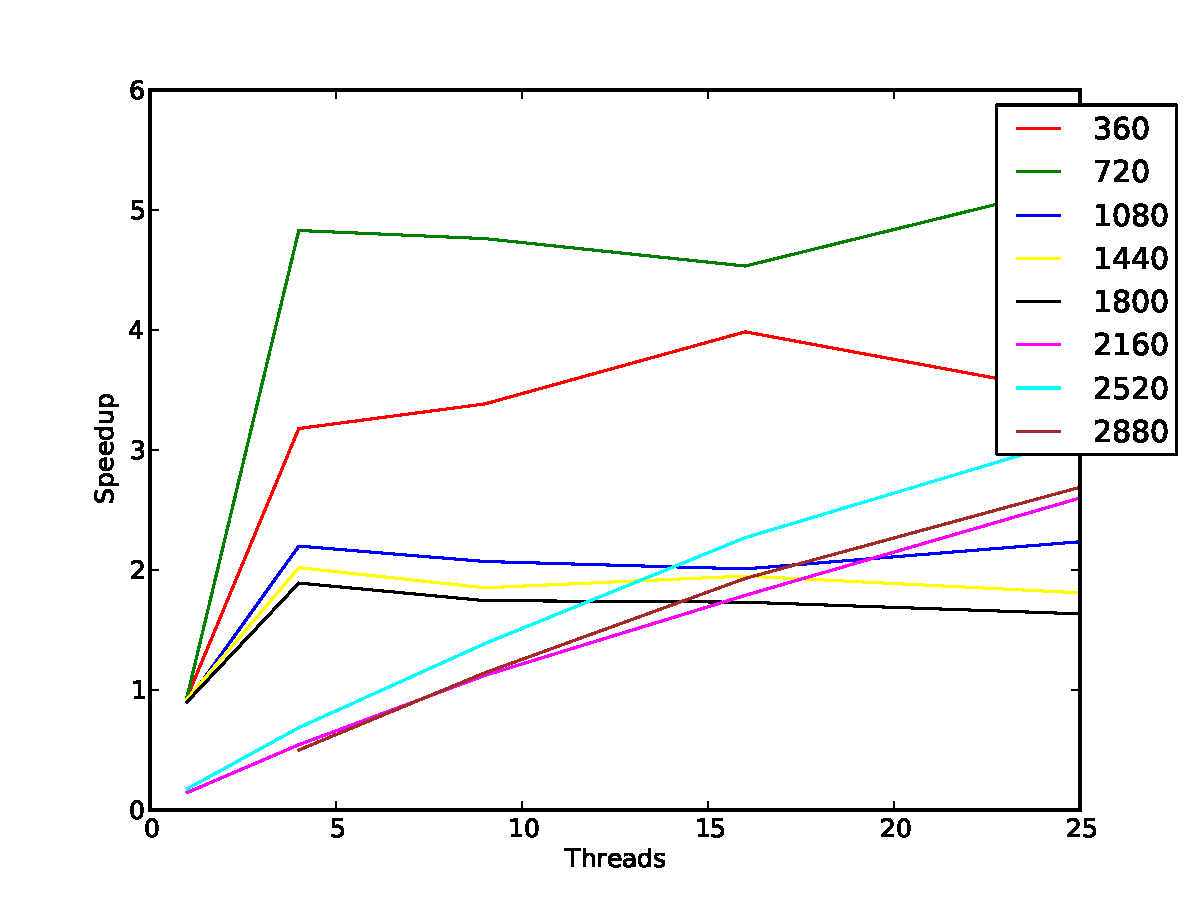
\includegraphics[width=0.5\linewidth]{e5_strong_bindel_baseline.pdf}
\caption{Strong scaling speedup for running on the Xeon E5 2620s. Baseline for calculating speedup is Professor Bindel's code from the point at which we forked it.}
\end{figure}

\begin{figure}[h!]
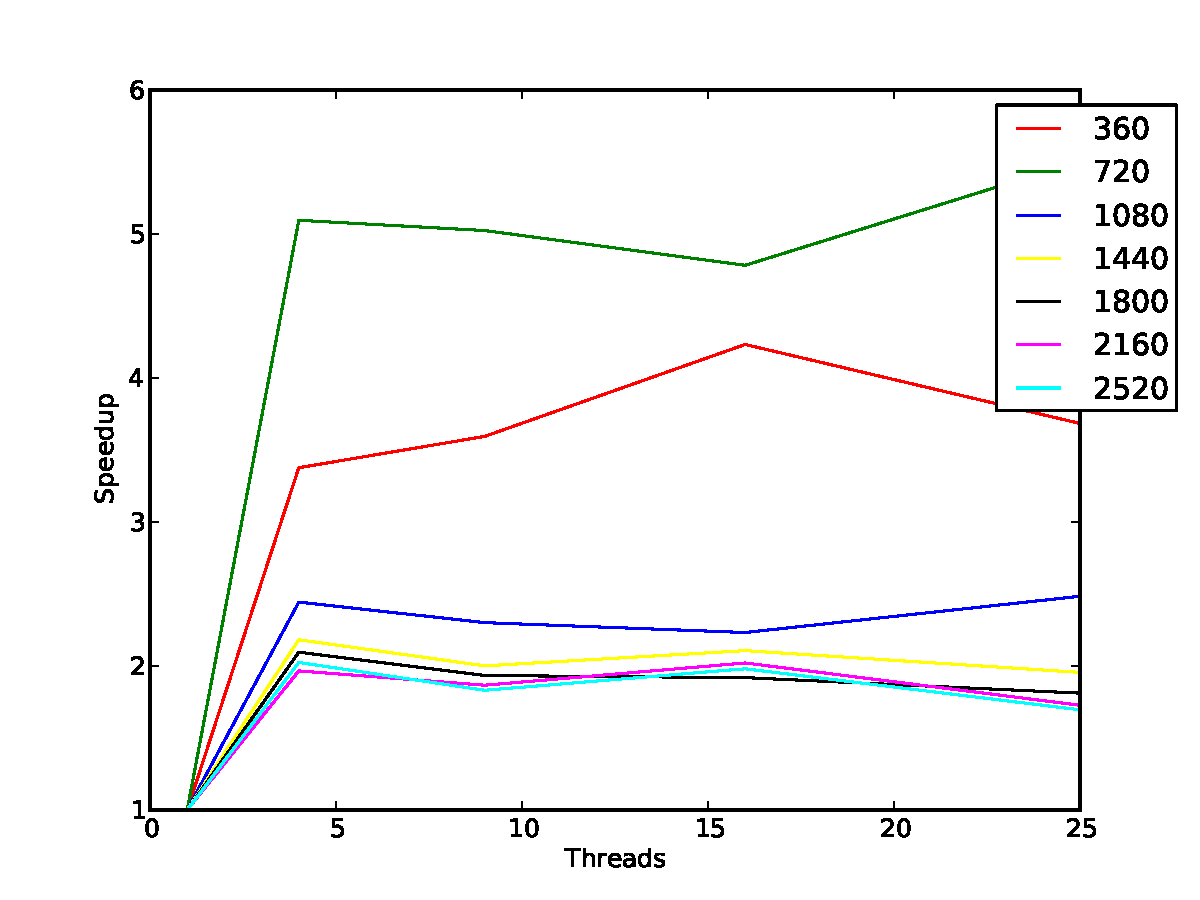
\includegraphics[width=0.5\linewidth]{e5_strong_e5_baseline.pdf}
\caption{Strong scaling speedup for running on the Xeon E5 2620s. Baseline for calculating speedup is our code running a single thread on the main node (Xeon E5 2620s).}
\end{figure}

\subsubsection{Weak Scaling}
\begin{figure}[h!]
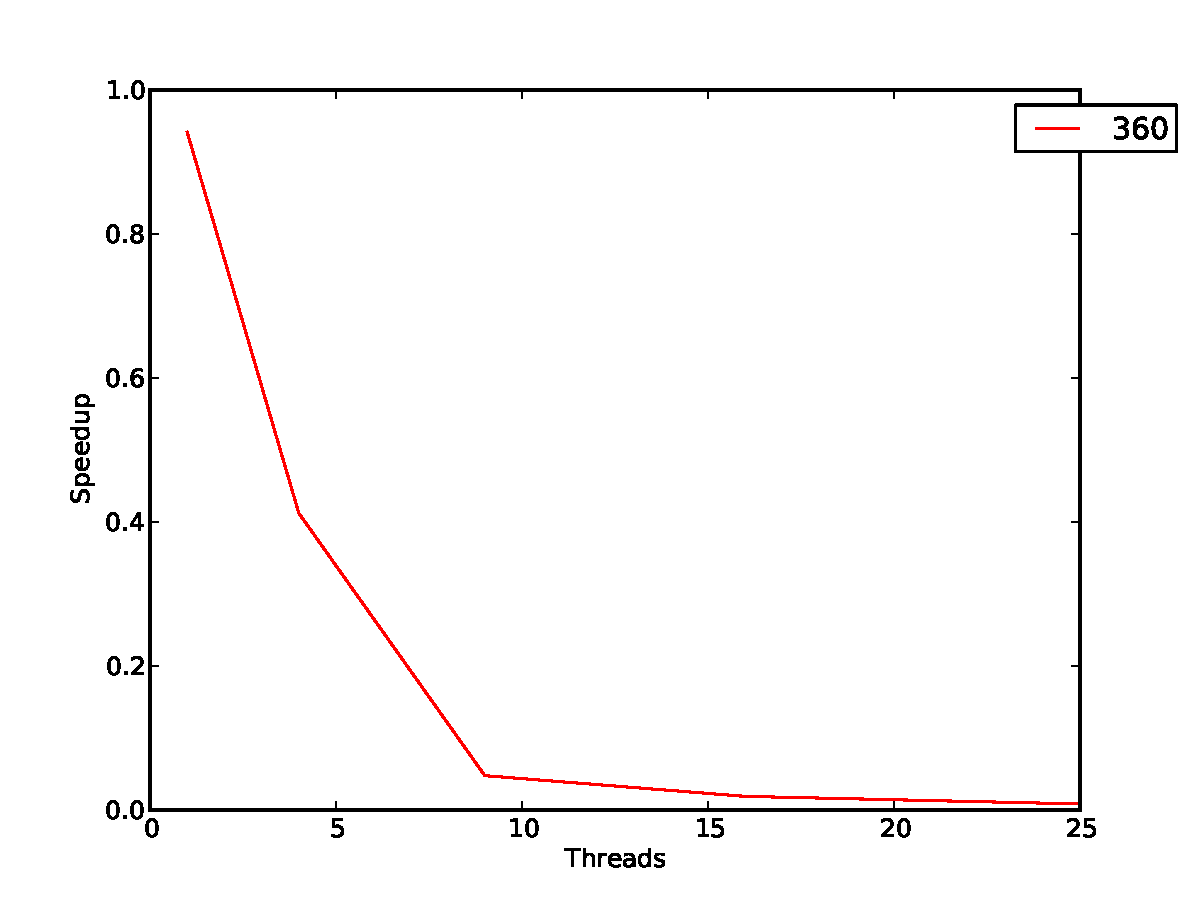
\includegraphics[width=0.5\linewidth]{e5_weak_bindel_baseline.pdf}
\caption{Weak scaling speedup for running on the Xeon E5 2620s. Baseline for calculating speedup is Professor Bindel's code from the point at which we forked it.}
\end{figure}

\begin{figure}[h!]
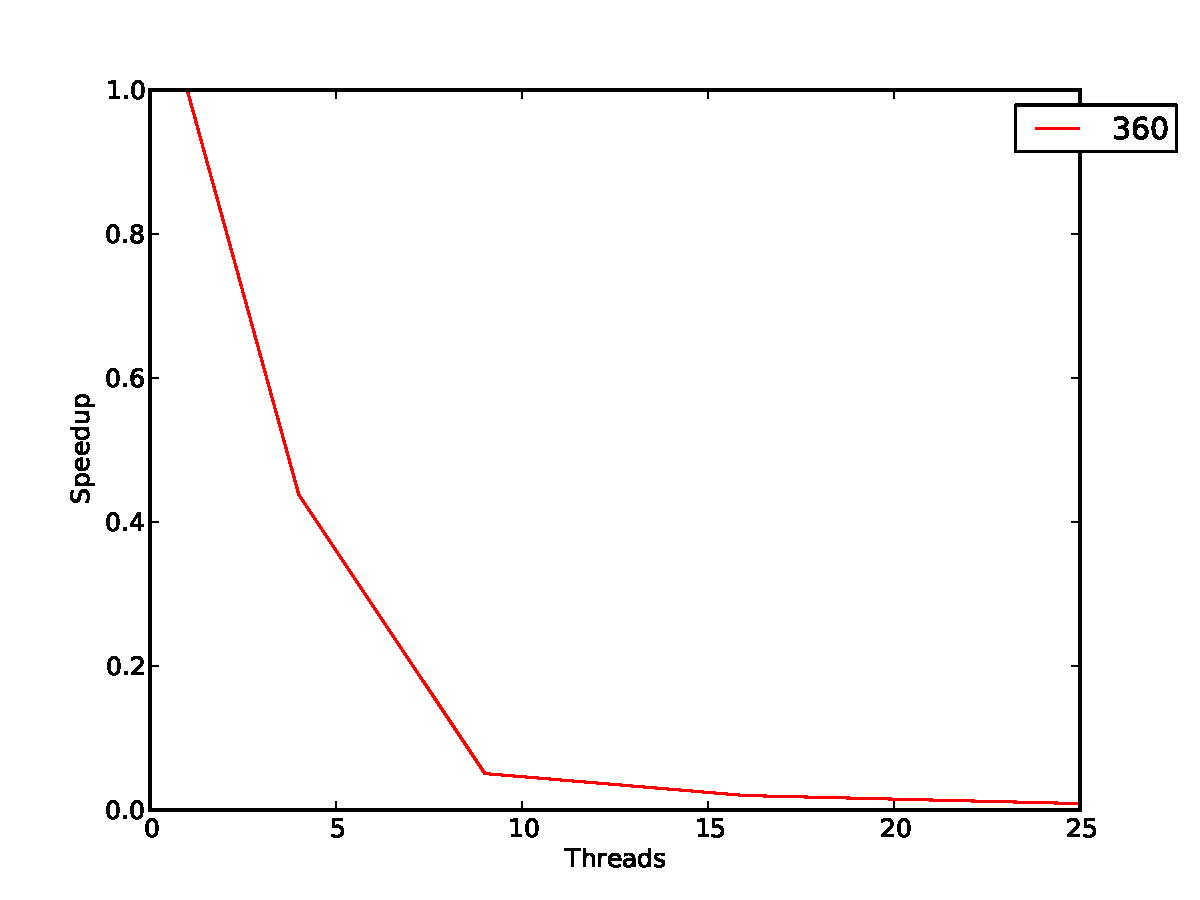
\includegraphics[width=0.5\linewidth]{e5_weak_e5_baseline.pdf}
\caption{Weak scaling speedup for our parallel code running on the Xeon E5 2620s. Baseline for calculating speedup is our code running a single thread on the main node (Xeon E5 2620s).}
\end{figure}

\subsection{Xeon Phi Performance}

\subsubsection{Strong Scaling}
\begin{figure}[h!]
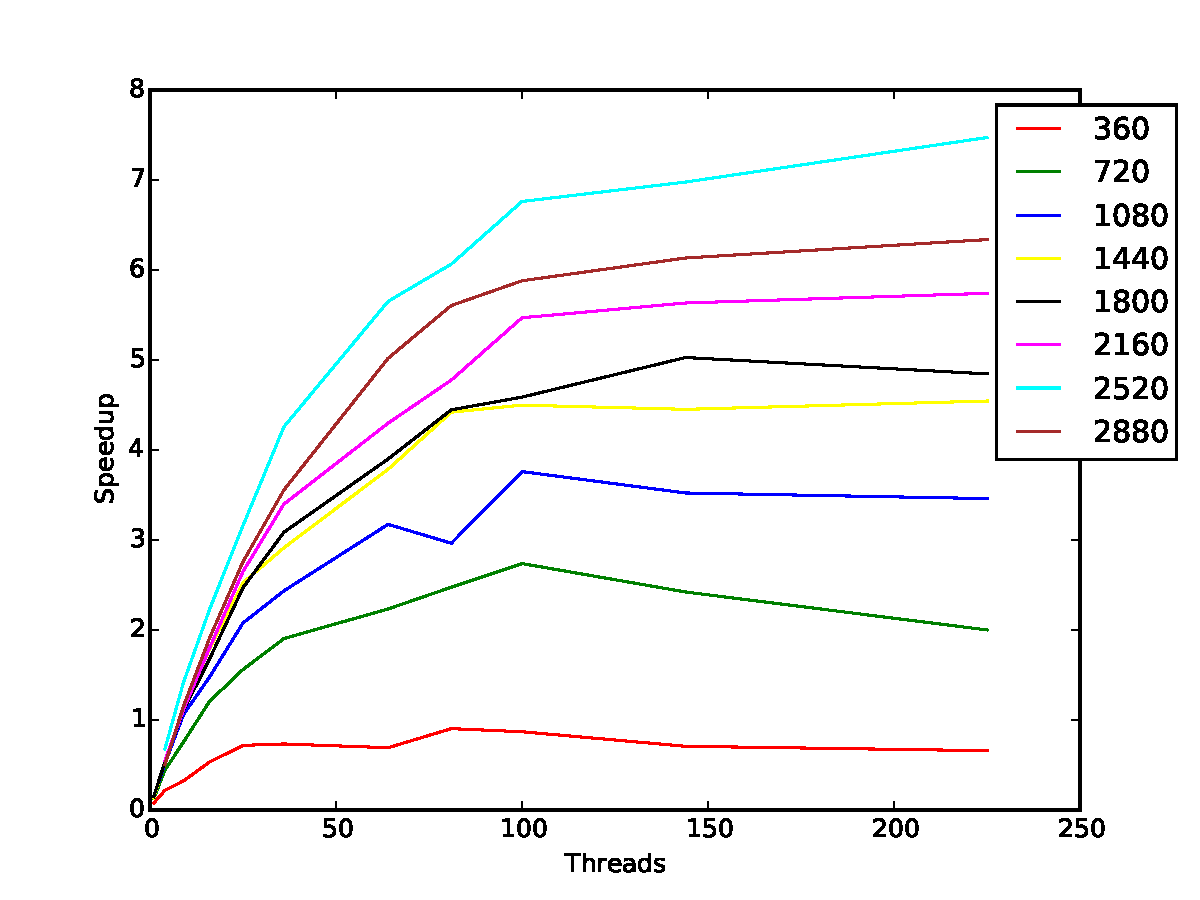
\includegraphics[width=0.5\linewidth]{mic_strong_bindel_baseline.pdf}
\caption{Strong scaling speedup for our offloaded Phi code. Baseline for calculating speedup is Professor Bindel's code from the point at which we forked it.}
\end{figure}

\begin{figure}[h!]
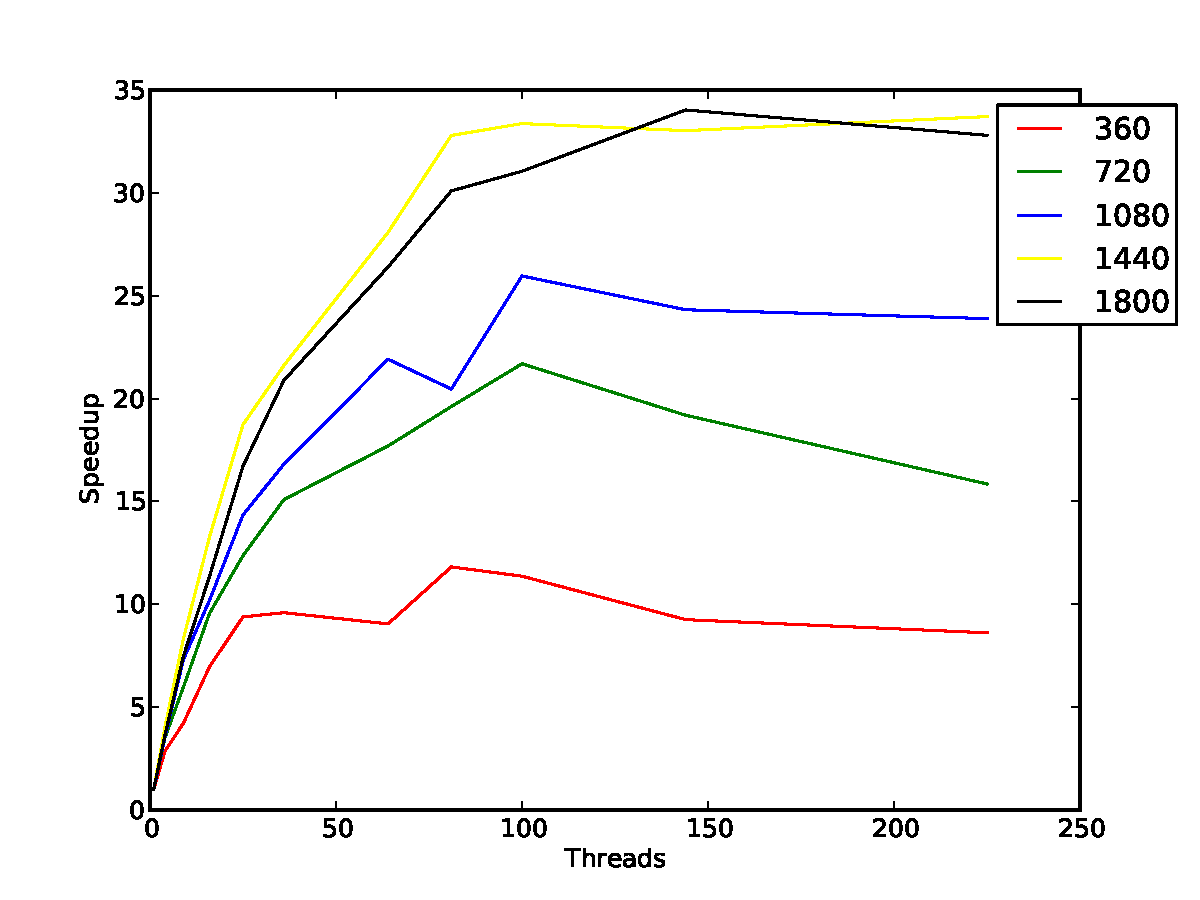
\includegraphics[width=0.5\linewidth]{mic_strong_mic_baseline.pdf}
\caption{Strong scaling speedup for our offloaded Phi code. Baseline for calculating speedup is our code running a single thread offloaded to the Phis.}
\end{figure}

\subsubsection{Weak Scaling}
\begin{figure}[h!]
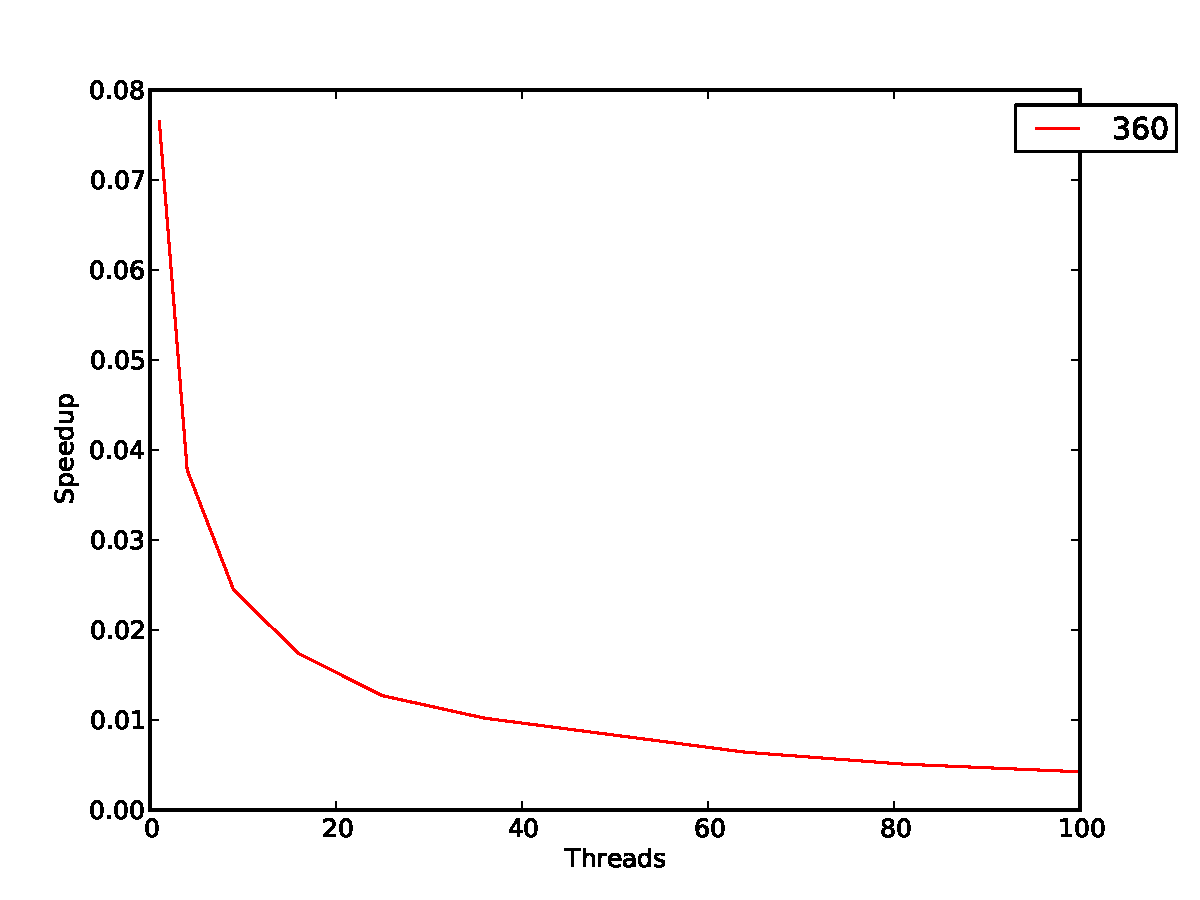
\includegraphics[width=0.5\linewidth]{mic_weak_bindel_baseline.pdf}
\caption{Weak scaling speedup for our offloaded Phi code. Baseline for calculating speedup is Professor Bindel's code from the point at which we forked it.}
\end{figure}

\begin{figure}[h!]
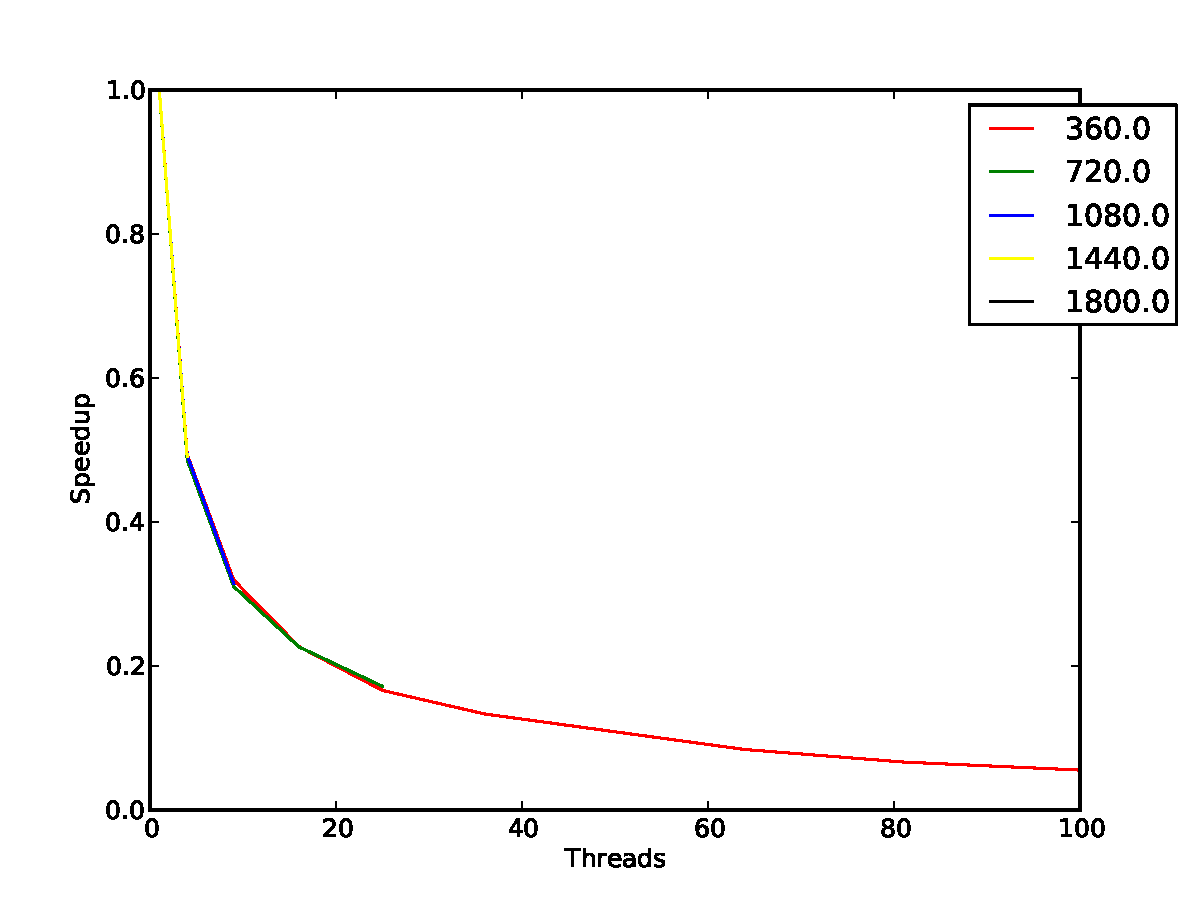
\includegraphics[width=0.5\linewidth]{mic_weak_mic_baseline.pdf}
\caption{Weak scaling speedup for our offloaded Phi code. Baseline for calculating speedup is our code running a single thread offloaded to the Phis.}
\end{figure}

\subsection{Batch size Performance}

We were also interested in how our code performed when we increased batch size on the Xeon Phi boards. We found that when we increased batch size to two rather than 1 (so 4 steps rather than 2 steps), that our total time was actually slightly worse. This is likely because there are few barriers in our code (one after our speed calculation, one after our copy and compute steps calculation, one after our synchronize section) and no single-threaded sections which take large computation time. Thus synchronization wasn't all the expensive and the extra work (in terms of more ghost cells that have to be calculated for) does not outweigh the decreased synchronization frequency.

Furthermore it is likely that because we have to back-off our dt when doing a batch size of moer than 1 in order to be conservative and not violate the CFL constraint we must do more steps total for our simulatino to complete which is more work. Further a larger batch size potentially leads to many extra steps taken near the end of a simulation when a smaller number of steps would suffice.

\begin{figure}[h!]
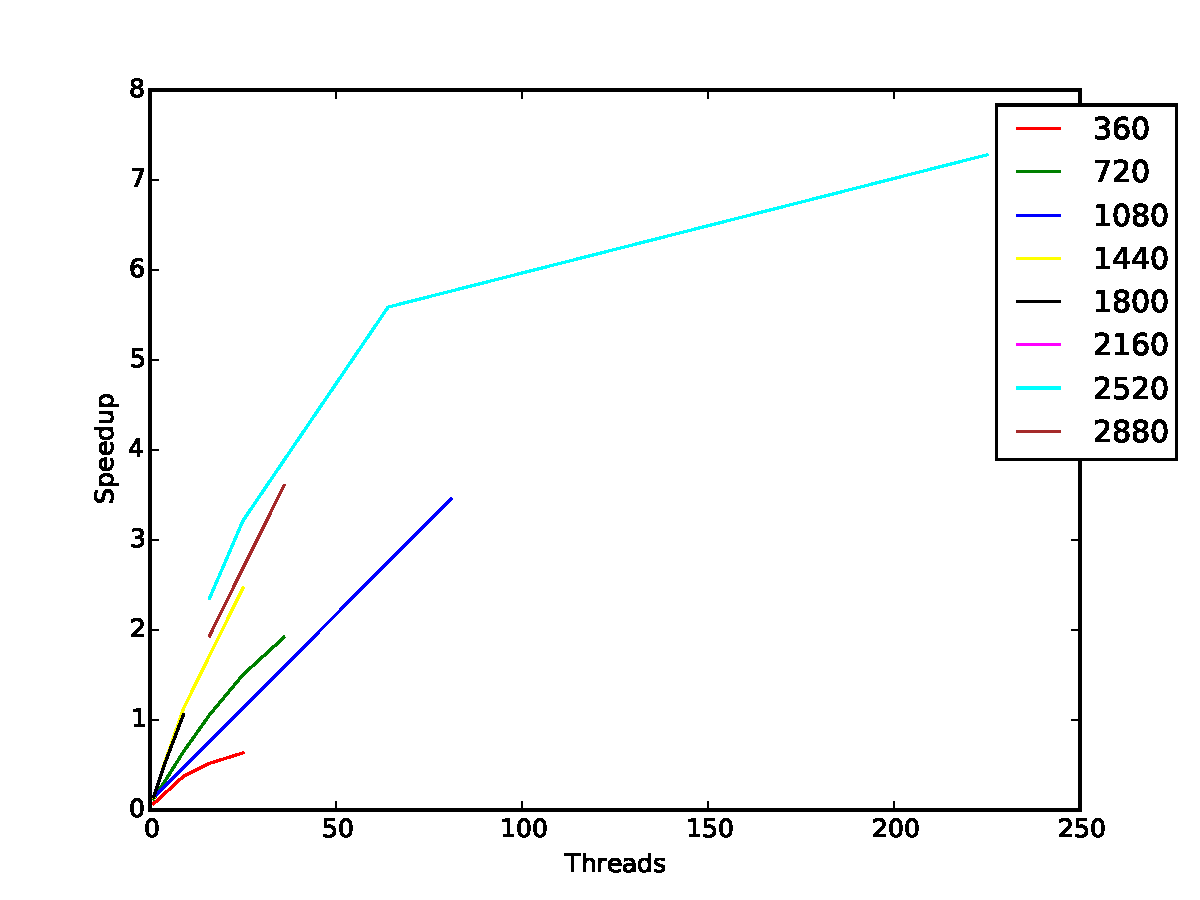
\includegraphics[width=0.5\linewidth]{mic_strong_bindel_baseline_batchsize2.pdf}
\caption{Strong scaling speedup for our offloaded Phi code with a batch size of 2. Baseline for calculating speedup is Professor Bindel's code at the point where we forked it. We can see that speedup is slightly worse than our speedup for batch size of 1.}
\end{figure}
